\section{Controllers}\label{sec:ContDiscrete}
To implement the controllers on the microcontroller they must first be transformed into the discrete domain.

This transformation is done through the Tustin (bilinear) approximation in which the $s$ term in the transfer function is substituted as seen in \autoref{tustin} \cite{tustin}.
\begin{flalign}
	s\approx\frac{2}{T}\frac{z-1}{z+1}
	\label{tustin}
\end{flalign}
\begin{where}
	\va{s}{is the Laplace operator}{}
	\va{z}{is the equivalent of the Laplace operator in discrete domain}{}
	\va{T}{is the sampling period}{s}
\end{where}
The Tustin method maps the Laplace stable region into the discrete stable region, that is, the unit circle, as seen in \autoref{fig:tustinmap}.
\begin{figure}[H]
	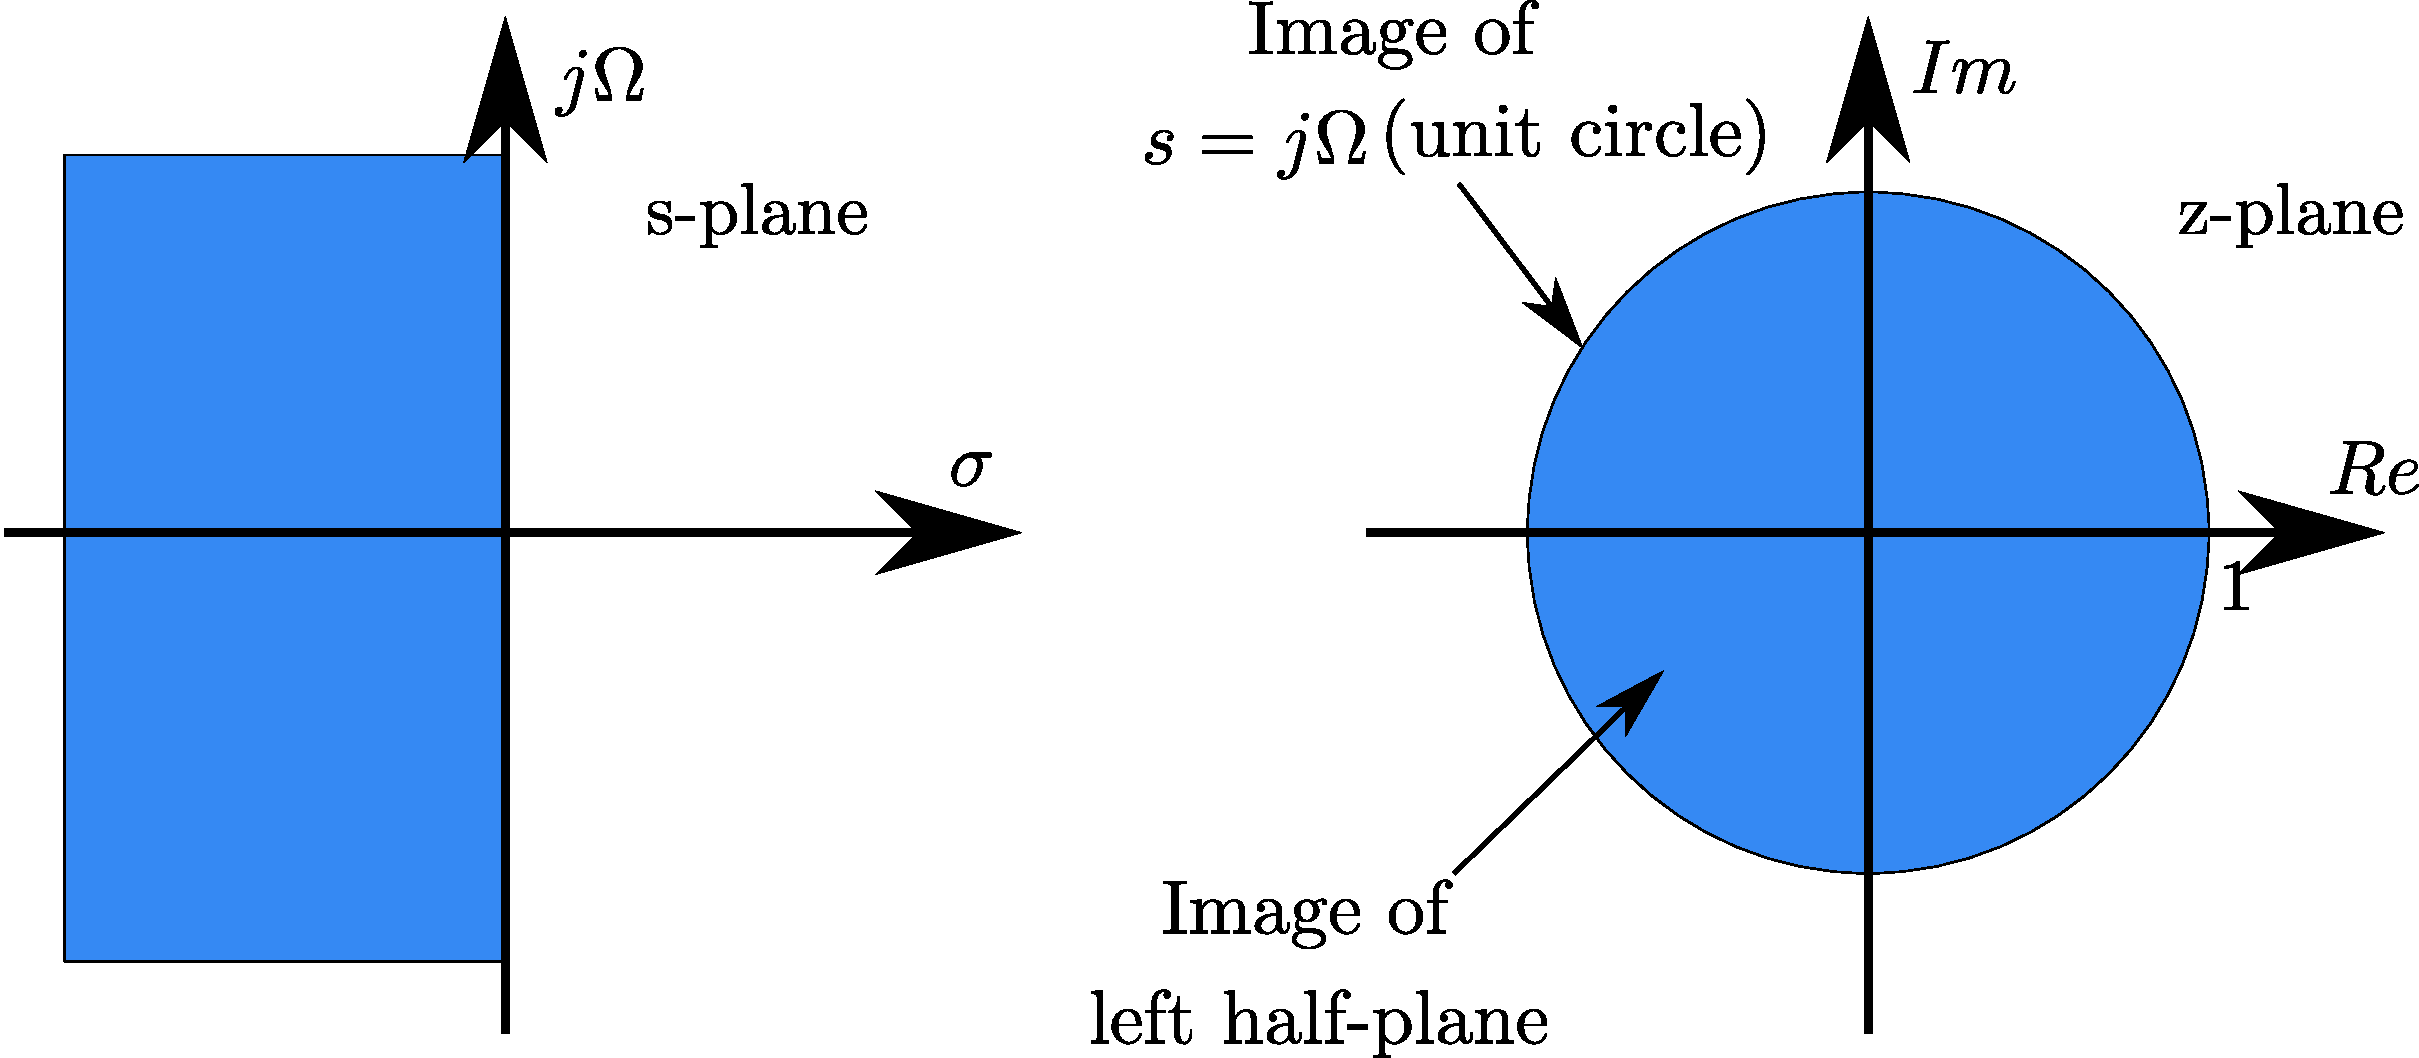
\includegraphics[scale=.25]{figures/S-planeVsZ-plane.pdf}
	\centering			
	\captionof{figure}{The s-domain and the z-domain \cite{AVOppenheim}.} 
	\label{fig:tustinmap}
\end{figure} 
The discrete transfer function is then transformed into a difference equation to obtain the expression to be applied in the microcontroller. This is done taking into account that a $z^{-1}$ term implies taking the previous sample of the data. 

When discretizing the controller, the sampling time must also be considered. In the system at hand, the sampling frequency is limited by the sensor data (Vicon System) to be 100 Hz as a maximum. To ensure that the discretization does not affect the controller response, the lower sampling limit is set taking into account the bandwidth of the controllers. To do so, the sampling frequency should be between 10 and 20 times higher than the bandwidth of the control loop. The fastest control loop in the system is the attitude controller, which has a bandwidth of 2 \si{rad\cdot s^{-1}}, that is, 0.32 Hz. This implies a minimum sampling frequency of 3.2 Hz.

The sampling period is chosen to be 0.035 ms, which is the fastest possible within the schedule as described in \autoref{sec:Scheduler}.
\subsection{Attitude Controller}
The attitude controller is mainly composed of gains formed by the state feedback, the integral and the observer matrices. This makes the discretization easier as there are no $s$-terms in the controller. There are however several integrators, three of which are in the observer and the remaining three in the integral part of the controller.

The discrete form of an integrator using the Tustin approximation is shown in \autoref{discreteIntegrator}. The formula shows the discretized version of the integrator in the integral term of the attitude control. The first relation in \autoref{discreteIntegrator} is obtained from \autoref{fig:DetailedControllerColorDiagram}.
\begin{flalign}
	\frac{x_\mathrm{int}}{e} = \frac{1}{s} \approx \frac{T}{2}\frac{z+1}{z-1}
	\label{discreteIntegrator}
\end{flalign}
This transformation yields a difference equation as seen in \autoref{discreteIntegratordifferences}. It gives the current value of the integral state as a function of the previous integral state, the current and the previous error between the angular reference and the angular data.
\begin{flalign}
	x_\mathrm{int}(k)=x_\mathrm{int}(k-1) + \frac{T}{2} e(k) + \frac{T}{2} e(k-1)
	\label{discreteIntegratordifferences}
\end{flalign}

%This approximation is used similarly in the rest of integrators present in the controller.
%The effect of the discretization in the designed attitude controllers has been simulated in the non-linear system and it is commpared with the continuous designed previously developed. See \autoref{fig:AttitudeDiscrete}. It can be seen that the discretized version of the controller makes it slower, but the overshoot is slightly reduced. There no change in the final value of the controller.
%\begin{figure}[H]
%	\centering
%	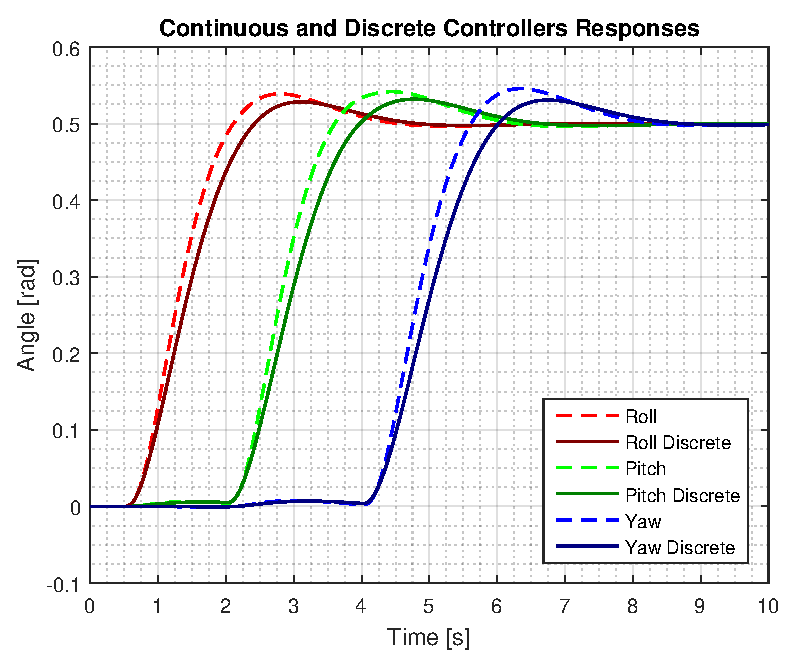
\includegraphics[scale=0.65]{figures/simAttitudeDiscrete}
%	\caption{Attitude controller performance when discretized with a sampling rate of 28 Hz and its continuous version.}
%	\label{fig:AttitudeDiscrete}
%\end{figure}
%
%The discrete attitude controller is also evaluated by its control action, which is depicted in \autoref{fig:AttitudeDiscreteControlAction}. As it can be appreciated, the variations from equilibrium of the motor rotational speeds are larger in the discrete controller and the signals are away from equilibrium for a longer time.
%\begin{figure}[H]
%	\centering
%	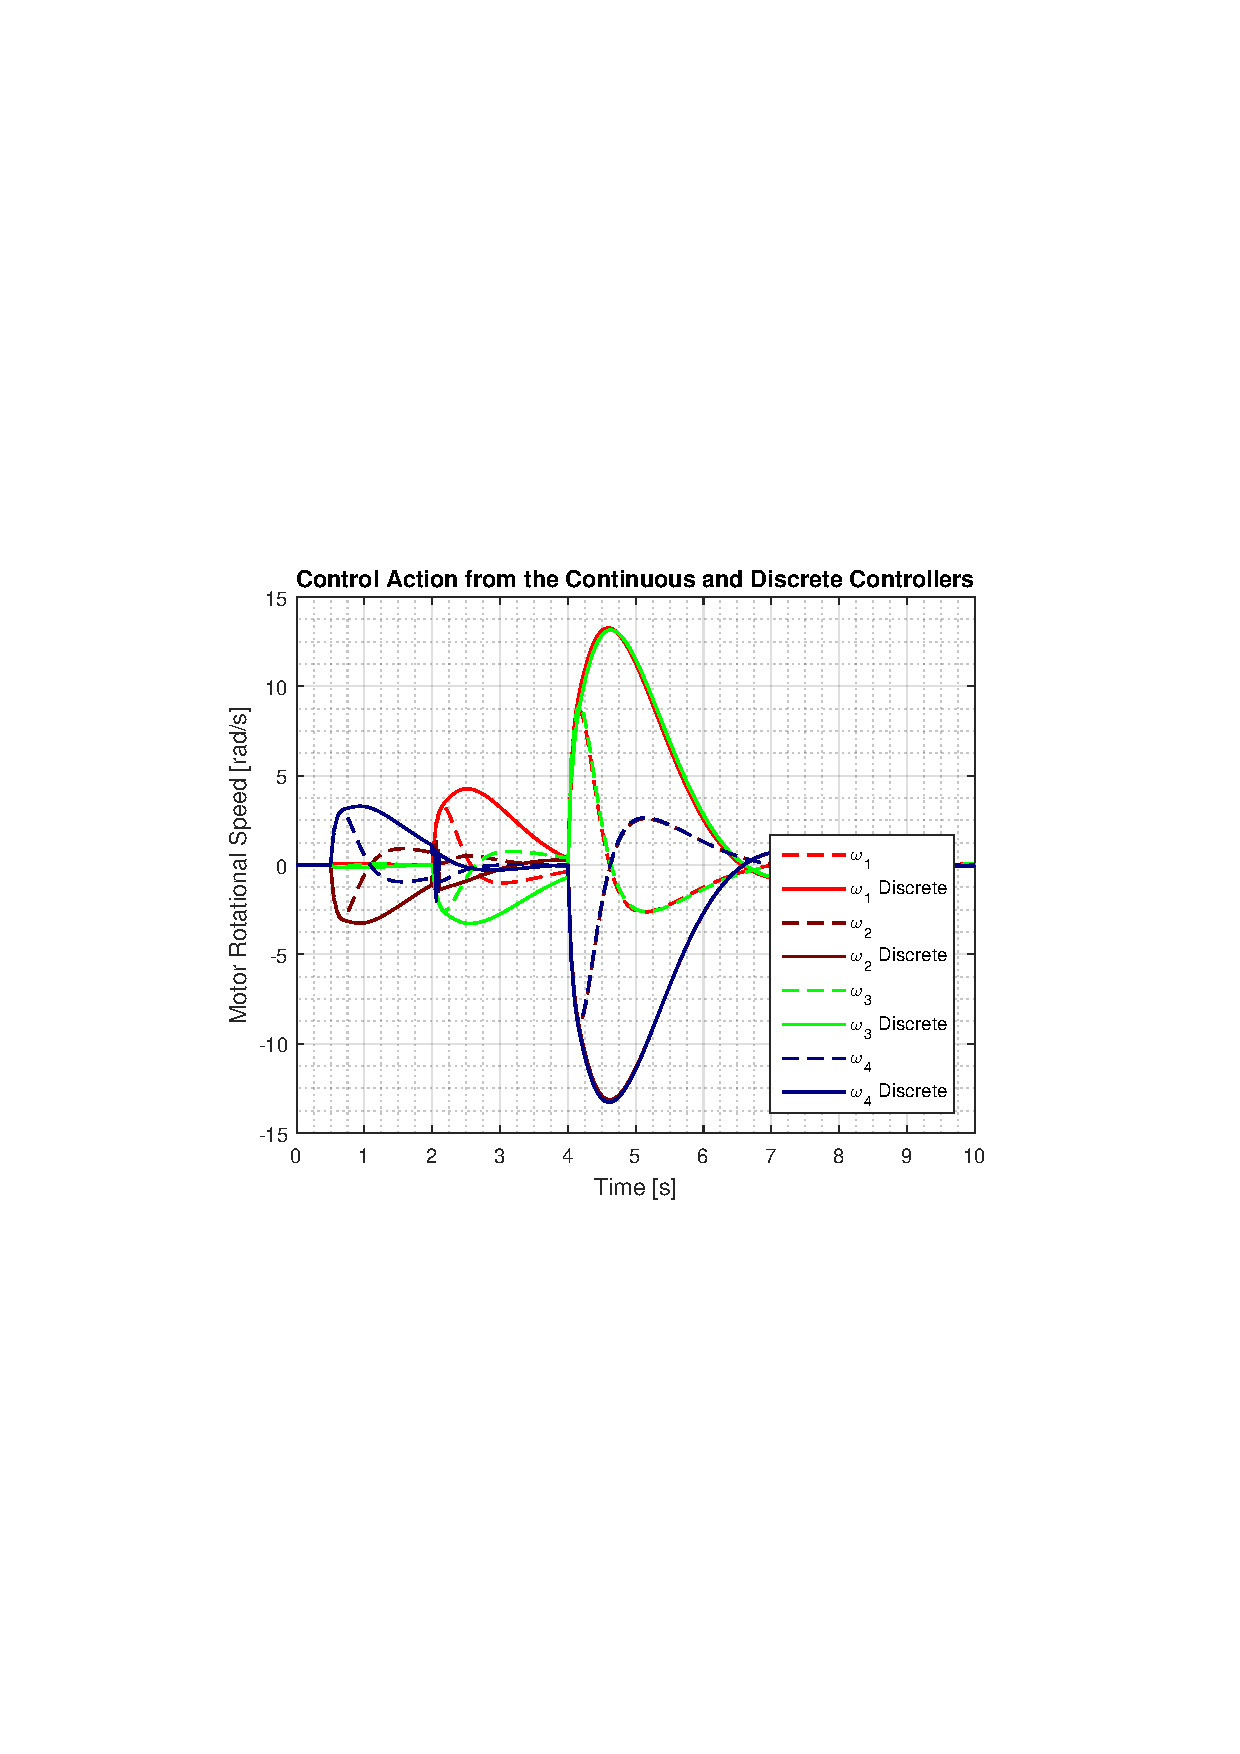
\includegraphics[scale=0.65]{figures/simAttitudeDiscreteControlAction}
%	\caption{Attitude controller control action when discretized with a sampling rate of 28 Hz and its continuous version.}
%	\label{fig:AttitudeDiscreteControlAction}
%\end{figure}
\subsection{Translational Controllers}
The translational position controllers contain only proportional terms, which means that no discretization is needed. However, the velocity controllers also include an integral term and therefore they need to be discretized. This is also done using the Tustin approximation, same as for the attitude controller.

The discrete versions of the PI controllers are 
\begin{flalign}
	\theta_{\mathrm{ref}}(k&)= \theta_{\mathrm{ref}}(k-1) -0.08 e_{\dot{x}}(k) + 0.08 e_{\dot{x}}(k-1)
	\label{discreteVelocityXcontrollerdiferences}\\
	\phi_{\mathrm{ref}}(k)&= \phi_{\mathrm{ref}}(k-1) +0.08 e_{\dot{y}}(k) -0.08 e_{\dot{y}}(k-1)
	\label{discreteVelocityYcontrollerdiferences}\\
	\omega_\mathrm{sum}(k)&= \omega_\mathrm{sum}(k-1) -283.9 e_{\dot{z}}(k) + 276.1 e_{\dot{z}}(k-1)
	\label{discreteVelocityZcontrollerdiferences}
\end{flalign}
\subsection{Controller Code}
As in the case of the communication, the controllers are included in a task that runs every sampling period, $T = 35$ \si{ms}. As seen in \autoref{lst:controllerTask} this is done by storing the time at which the task starts in the variable \lstinline[style=customcppinline]{xLastWakeTime}. This is then used in the function \lstinline[style=customcppinline]{vTaskDelayUntil()} to count 35 ms from \lstinline[style=customcppinline]{xLastWakeTime} before the control task is run again. For each period the control code is executed and the calculated control actions are send to the motor controllers in the form of a PWM signal.



\begin{lstlisting}[style=customcpp,
caption={Code for the controller task.}, 
label=lst:controllerTask]
void Controllers(void *pvParameters)
{ 
	// Variable to make the task periodic
	portTickType xLastWakeTime;
	// xTaskGetTickCount() returns start time of the task
	xLastWakeTime = xTaskGetTickCount();
	
	while (1)
	{
		Controller();
		ApplyVelocities();
		// A delay of 35 ms is set since the task started until the next task
		vTaskDelayUntil(&xLastWakeTime, 35);
	}
	vTaskDelete(NULL);
}
\end{lstlisting}

The implementation of the difference equations inside the function \lstinline[style=customcppinline]{Controllers()} is seen in \autoref{lst:controllers}, in which three examples , $\dot{z}_{\mathrm{I}}$ controller, integration in the state space controller and in the observer, are presented.

\begin{lstlisting}[style=customcpp,
caption={Code for the controllers.}, 
label=lst:controllers]
...
r_k[1] = -0.08*vel_e_k[0] + 0.08*vel_e_k1[0] + r_k[1]; // x velocity controller
...
r_k[0] = 0.08*vel_e_k[1] - 0.08*vel_e_k1[1] + r_k[0]; // y velocity controller
...
u_z = -283.9*vel_e_k[2] + 276.1*vel_e_k1[2] + u_z; // z velocity controller
...
xint_k[i] = T / 2 * (e_k[i] + e_k1[i]) + xint_k1[i]; // Integral control integrator
...
oint_k[i] = T / 2 * (o_k[i] + o_k1[i]) + oint_k1[i]; // Observer integrator
...

\end{lstlisting}

The function \lstinline[style=customcppinline]{ApplyVelocities()}, seen in \autoref{lst:controllerTask}, is in charge of mixing the control action of the attitude controller with the one coming from the $z_{\mathrm{I}}$ controller. Then the duties that correspond to the desired rotational speeds of the motor are calculated using the information of \autoref{app:duty} and the PWM signal is sent to the motor controllers.











